\section*{Technical Appendices and Supplementary Material}


\section{Benchmark Datasets}\label{sec:bench_datasets}

Table~\ref{tab:capabilities-benchmarks} summarizes the benchmark suite used to
evaluate each capability. For capabilities associated with multiple benchmarks,
we report the average score across the listed benchmarks.


\begin{table}[h]
  \centering
  \caption{Benchmark suite for evaluating LLM capabilities.}
  \label{tab:capabilities-benchmarks}
  \small
  \setlength{\tabcolsep}{4pt}
  \renewcommand{\arraystretch}{0.95}

  \begin{tabularx}{\linewidth}{@{}
    >{\raggedright\arraybackslash}p{0.20\linewidth}
    >{\raggedright\arraybackslash}p{0.36\linewidth}
    >{\raggedright\arraybackslash}X
  @{}}
    \toprule
    \textbf{Capability} & \textbf{Benchmarks} & \textbf{Metric} \\
    \midrule
    General      & MMLU-Pro, BIG       & Accuracy \\
    Steerability & IFEval, FollowEval  & Instruction-following accuracy \\
    Reasoning    & GPQA, ARC-Challenge & Normalized accuracy \\
    Math         & MATH Hard, GSM8K    & Exact match \\
    Code         & HumanEval, MBPP     & Pass@1 \\
    Tool Use     & BFCL V4, ToolBench  & Tool-call success rate \\
    LCU          & LongBench           & Average normalized score \\
    Multilingual & XCOPA, MGSM         & Macro accuracy \\
    \bottomrule
  \end{tabularx}
\end{table}

\begin{itemize}
    \item \textbf{MMLU-Pro}~\citep{wang2024mmluprorobustchallengingmultitask} tests broad knowledge and problem-solving across many academic subjects using multiple-choice questions. 
    \item \textbf{BIG-bench (BIG)}~\citep{suzgun2022challenging} is a large collection of diverse tasks designed to probe general reasoning and knowledge beyond standard exams.
    \item \textbf{IFEval}~\citep{zhou2023instructionfollowing} measures instruction following by checking whether model outputs satisfy explicit, verifiable constraints in the prompt.
    \item \textbf{FollowEval}~\citep{jing2023followeval} evaluates how well a model follows user instructions under varied formats and constraint types, complementing IFEval with broader instruction patterns.
    \item \textbf{GPQA}~\citep{rein2024gpqa} is a graduate-level question answering benchmark that stresses hard scientific reasoning with high-quality, expert-written questions.
    \item \textbf{ARC-Challenge}~\citep{Clark2018ThinkYH} contains difficult grade-school science questions that require multi-step reasoning and commonsense beyond keyword matching.
    \item \textbf{MATH Hard}~\citep{hendrycksmath2021} is a challenging subset of competition-style math problems and is scored by exact final-answer match.
    \item \textbf{GSM8K}~\citep{cobbe2021training} focuses on grade-school math word problems that require intermediate reasoning steps, also scored by exact final-answer match.
    \item \textbf{HumanEval}~\citep{chen2021codex} evaluates code generation via functional correctness on hand-written programming problems, reported as Pass@1.
    \item \textbf{MBPP}~\citep{austin2021program} is a Python programming benchmark with short programming tasks and unit tests, also evaluated by Pass@1.
    \item \textbf{BFCL V4}~\citep{berkeley-function-calling-leaderboard} measures tool-use ability by checking whether the model can produce correct function calls under realistic tool specifications.
    \item \textbf{ToolBench}~\citep{xu2023tool} evaluates tool use in more complex, multi-tool scenarios and is scored by tool-call success rate.
    \item \textbf{LongBench}~\citep{bai2024longbench} evaluates long-context understanding across multiple long-input tasks and reports an average normalized score.
    \item \textbf{XCOPA}~\citep{ponti2020xcopa} tests multilingual causal commonsense reasoning across languages and is reported using macro accuracy.
    \item \textbf{MGSM}~\citep{shi2022language} is a multilingual version of grade-school math and is evaluated by macro accuracy across languages.
\end{itemize}

\section{Empirical Study Setting}\label{sec:app_em}

We study capability interactions under a fixed distillation budget by distilling a student model toward one target capability at a time and then evaluating the resulting student on \emph{all} capabilities in Table~\ref{tab:capabilities-benchmarks}. 
For each capability, we build a capability-specific distillation pool from the corresponding benchmark prompts, excluding any held-out evaluation examples to prevent leakage. 
We repeat this process under multiple token budgets (e.g., 20M, 80M, 150M tokens) to form a budget-dependent capability transfer matrix, where each entry is the score change on a destination capability when distilling toward a source capability at budget $B$. 
We use deterministic decoding for generation benchmarks (temperature $=0$) with a fixed prompt template across methods, and we compute each capability score as the average over its associated benchmarks in the table. We instantiate a simple but representative set of capability distillation baselines by combining three supervision forms that expose different levels of teacher knowledge---\textit{Resp} (final answer only), \textit{CoT} (rationale plus final answer), and \textit{Logit} (token-level soft targets)—with two standard objectives, \textit{SFT} and \textit{KD}, yielding six baselines in total.

\section{Additional Theoretical Analysis}\label{sec:app_theory}
\textbf{Uncertainty-aware UCB allocation}. Here, we conduct an uncertainty-aware UCB allocation analysis showing that action-level regret is controlled by predictive uncertainty. At interval $t$, ReAD maintains a bandit context
\begin{equation}
\mathbf{x}_t := [\,\mathbf{r}_\tau;\ \mathbf{s}(S_{t});\ b_t\,],
\label{eq:context_short}
\end{equation}
where $\mathbf{r}_\tau\in\Delta$ is the task requirement vector, $\mathbf{s}(S_{t})\in\mathbb{R}^{|\mathcal{C}|}$ is the probe-defined capability profile of the current student, and $b_t$ is the remaining budget. Let $\mathcal{A}(\tau)$ be the discrete candidate action set of allocation vectors. Define the conditional expected proxy reward
\begin{equation}
\bar R(\mathbf{x},\mathbf{w}) := \mathbb{E}\!\left[\widehat{R}_t\mid \mathbf{x}_t=\mathbf{x},\ \mathbf{w}_t=\mathbf{w}\right],
\label{eq:expected_reward_short}
\end{equation}
where $\widehat{R}_t$ is the proxy reward used as shown in Eq.~\eqref{eq:reward}.

\begin{assumption}[Calibrated uncertainty]\label{ass:calibrated_uncertainty}
    For a confidence level $\delta\in(0,1)$, with probability at least $1-\delta$, for all encountered $(\mathbf{x}_t,\mathbf{w})$,
\begin{equation}
\big|\mu(\mathbf{x}_t,\mathbf{w})-\bar R(\mathbf{x}_t,\mathbf{w})\big| \le \sigma(\mathbf{x}_t,\mathbf{w}),
\label{eq:calibration_short}
\end{equation}
where $\mu$ and $\sigma$ are the ensemble mean and standard deviation defined from the reward regressors.
\end{assumption}

Since ReAD selects allocations by the UCB rule in Eq.~\eqref{eq:ucb}, we can compare its chosen action $\mathbf{w}_t$ to the optimal action $\mathbf{w}_t^\star$ under the same context and bound the resulting gap in conditional expected reward using the calibrated uncertainty condition in Assumption~\ref{ass:calibrated_uncertainty}, which leads to the following instantaneous regret bound.

\begin{proposition}[Instantaneous regret bound]
    Let $\mathbf{w}_t^\star\in\arg\max_{\mathbf{w}\in\mathcal{A}(\tau)} \bar R(\mathbf{x}_t,\mathbf{w})$. Under Assumption~\ref{ass:calibrated_uncertainty},
\begin{equation}
\bar R(\mathbf{x}_t,\mathbf{w}_t^\star)-\bar R(\mathbf{x}_t,\mathbf{w}_t)\ \le\ 2\kappa\,\sigma(\mathbf{x}_t,\mathbf{w}_t),
\label{eq:inst_regret_short}
\end{equation}
and consequently,
\begin{equation}
\sum_{t=1}^T \Big(\bar R(\mathbf{x}_t,\mathbf{w}_t^\star)-\bar R(\mathbf{x}_t,\mathbf{w}_t)\Big)
\ \le\ 2\kappa\sum_{t=1}^T \sigma(\mathbf{x}_t,\mathbf{w}_t).
\label{eq:cum_regret_short}
\end{equation}
\end{proposition}

\section{Additional Experiments}\label{sec:app_experiment}

\begin{table*}[t]
\centering
\tiny
\setlength\tabcolsep{1pt}
\caption{Capability profile of different methods under a 150M-token budget (LLama). ReAD consistently outperforms all six baselines.}
\begin{tabular}{lcccccccc}
\toprule
\textbf{Method} &
\textbf{General} &
\textbf{Steerability} &
\textbf{Reasoning} &
\textbf{Math} &
\textbf{Code} &
\textbf{Tool Use} &
\textbf{LCU} &
\textbf{Multilingual} \\
\midrule
Teacher only &
$48.13\pm0.35$ &
$89.98\pm0.40$ &
$10.51\pm0.12$ &
$48.34\pm0.55$ &
$88.40\pm0.70$ &
$31.90\pm0.45$ &
$36.20\pm0.40$ &
$91.10\pm0.55$ \\
Student only &
$31.09\pm0.40$ &
$49.22\pm0.55$ &
$8.72\pm0.15$ &
$15.56\pm0.60$ &
$72.60\pm0.95$ &
$25.83\pm0.60$ &
$30.40\pm0.45$ &
$68.90\pm0.80$ \\
\midrule
Resp-SFT &
$38.41\pm0.58$ &
$68.73\pm0.94$ &
$9.55\pm0.14$ &
$28.72\pm1.08$ &
$79.18\pm1.26$ &
$28.53\pm0.82$ &
$32.69\pm0.73$ &
$78.23\pm1.12$ \\
CoT-SFT &
$38.02\pm0.61$ &
$67.92\pm0.89$ &
$10.14\pm0.12$ &
$31.58\pm0.97$ &
$78.86\pm1.33$ &
$28.41\pm0.79$ &
$32.83\pm0.68$ &
$77.77\pm1.06$ \\
Logit-SFT &
$39.03\pm0.56$ &
$69.38\pm0.86$ &
$9.70\pm0.13$ &
$29.61\pm1.02$ &
$79.69\pm1.21$ &
$28.71\pm0.77$ &
$33.01\pm0.70$ &
$78.63\pm1.09$ \\
Resp-KD &
$39.62\pm0.53$ &
$70.98\pm0.84$ &
$9.82\pm0.12$ &
$30.21\pm0.98$ &
$80.09\pm1.18$ &
$29.09\pm0.74$ &
$33.42\pm0.66$ &
$79.18\pm1.03$ \\
CoT-KD &
$39.12\pm0.55$ &
$69.84\pm0.88$ &
$10.26\pm0.11$ &
$33.02\pm0.92$ &
$79.81\pm1.24$ &
$29.01\pm0.71$ &
$33.19\pm0.69$ &
$78.71\pm1.01$ \\
Logit-KD &
$40.18\pm0.51$ &
$72.63\pm0.79$ &
$9.95\pm0.12$ &
$31.36\pm0.95$ &
$80.57\pm1.16$ &
$29.48\pm0.69$ &
$33.73\pm0.64$ &
$79.97\pm0.97$ \\
\midrule
\textbf{ReAD} &
$\mathbf{41.80\pm0.45}$ &
$\mathbf{78.20\pm0.70}$ &
$\mathbf{10.40\pm0.10}$ &
$\mathbf{35.20\pm0.80}$ &
$\mathbf{83.90\pm1.00}$ &
$\mathbf{31.30\pm0.55}$ &
$\mathbf{35.60\pm0.55}$ &
$\mathbf{84.10\pm0.90}$ \\
\bottomrule
\end{tabular}
\label{tab:llama_150m}
\end{table*}

% ----------------------------- Qwen: B = 20M -----------------------------
\begin{table*}[t]
\centering
\tiny
\setlength\tabcolsep{1pt}
\caption{Capability profile of different methods under a 20M-token budget (Qwen). ReAD consistently outperforms all six baselines.}
\begin{tabular}{lcccccccc}
\toprule
\textbf{Method} &
\textbf{General} &
\textbf{Steerability} &
\textbf{Reasoning} &
\textbf{Math} &
\textbf{Code} &
\textbf{Tool Use} &
\textbf{LCU} &
\textbf{Multilingual} \\
\midrule
Teacher only &
$55.27 \pm 0.46$ &
$92.36 \pm 0.52$ &
$14.28 \pm 0.18$ &
$55.74 \pm 0.78$ &
$90.12 \pm 0.88$ &
$36.08 \pm 0.63$ &
$40.23 \pm 0.57$ &
$92.34 \pm 0.66$ \\
Student only &
$40.07 \pm 0.61$ &
$70.18 \pm 0.74$ &
$11.47 \pm 0.22$ &
$28.26 \pm 0.95$ &
$81.96 \pm 1.10$ &
$30.06 \pm 0.82$ &
$34.17 \pm 0.71$ &
$83.14 \pm 0.93$ \\
\midrule
Resp-SFT &
$42.18 \pm 0.86$ &
$72.92 \pm 0.98$ &
$11.62 \pm 0.24$ &
$31.42 \pm 1.35$ &
$83.88 \pm 1.42$ &
$30.96 \pm 0.97$ &
$35.04 \pm 0.88$ &
$84.36 \pm 1.21$ \\
CoT-SFT &
$41.93 \pm 0.90$ &
$72.41 \pm 1.02$ &
$12.06 \pm 0.21$ &
$33.12 \pm 1.28$ &
$83.54 \pm 1.50$ &
$30.74 \pm 0.95$ &
$34.92 \pm 0.91$ &
$84.09 \pm 1.18$ \\
Logit-SFT &
$42.57 \pm 0.82$ &
$73.56 \pm 0.95$ &
$11.81 \pm 0.23$ &
$32.24 \pm 1.22$ &
$84.06 \pm 1.37$ &
$31.13 \pm 0.93$ &
$35.21 \pm 0.86$ &
$84.58 \pm 1.16$ \\
Resp-KD &
$42.79 \pm 0.80$ &
$74.03 \pm 0.92$ &
$11.93 \pm 0.22$ &
$32.68 \pm 1.18$ &
$84.22 \pm 1.30$ &
$31.42 \pm 0.90$ &
$35.44 \pm 0.83$ &
$84.92 \pm 1.10$ \\
CoT-KD &
$42.44 \pm 0.83$ &
$73.37 \pm 0.94$ &
$12.31 \pm 0.19$ &
$34.08 \pm 1.12$ &
$83.91 \pm 1.28$ &
$31.02 \pm 0.88$ &
$35.29 \pm 0.85$ &
$84.76 \pm 1.08$ \\
Logit-KD &
$43.06 \pm 0.78$ &
$74.74 \pm 0.88$ &
$12.04 \pm 0.21$ &
$33.07 \pm 1.10$ &
$84.55 \pm 1.22$ &
$31.77 \pm 0.86$ &
$35.73 \pm 0.80$ &
$85.27 \pm 1.02$ \\
\midrule
\textbf{ReAD} &
$\mathbf{44.63 \pm 0.73}$ &
$\mathbf{78.57 \pm 0.86}$ &
$\mathbf{12.86 \pm 0.17}$ &
$\mathbf{36.24 \pm 1.05}$ &
$\mathbf{86.38 \pm 1.18}$ &
$\mathbf{33.41 \pm 0.79}$ &
$\mathbf{36.98 \pm 0.77}$ &
$\mathbf{87.23 \pm 0.95}$ \\
\bottomrule
\end{tabular}
\label{tab:qwen_20m}
\end{table*}


\begin{table*}[t]
\centering
\tiny
\setlength\tabcolsep{1pt}
\caption{Capability profile of different methods under a 150M-token budget (Qwen). ReAD consistently outperforms all six baselines.}
\begin{tabular}{lcccccccc}
\toprule
\textbf{Method} &
\textbf{General} &
\textbf{Steerability} &
\textbf{Reasoning} &
\textbf{Math} &
\textbf{Code} &
\textbf{Tool Use} &
\textbf{LCU} &
\textbf{Multilingual} \\
\midrule
Teacher only &
$55.27 \pm 0.46$ &
$92.36 \pm 0.52$ &
$14.28 \pm 0.18$ &
$55.74 \pm 0.78$ &
$90.12 \pm 0.88$ &
$36.08 \pm 0.63$ &
$40.23 \pm 0.57$ &
$92.34 \pm 0.66$ \\
Student only &
$40.07 \pm 0.61$ &
$70.18 \pm 0.74$ &
$11.47 \pm 0.22$ &
$28.26 \pm 0.95$ &
$81.96 \pm 1.10$ &
$30.06 \pm 0.82$ &
$34.17 \pm 0.71$ &
$83.14 \pm 0.93$ \\
\midrule
Resp-SFT &
$48.02 \pm 0.92$ &
$82.07 \pm 1.04$ &
$13.18 \pm 0.20$ &
$41.26 \pm 1.38$ &
$86.92 \pm 1.40$ &
$33.29 \pm 0.96$ &
$37.42 \pm 0.88$ &
$88.07 \pm 1.20$ \\
CoT-SFT &
$48.29 \pm 0.88$ &
$82.61 \pm 0.98$ &
$13.72 \pm 0.18$ &
$44.43 \pm 1.30$ &
$86.58 \pm 1.45$ &
$33.05 \pm 0.94$ &
$37.28 \pm 0.90$ &
$87.96 \pm 1.18$ \\
Logit-SFT &
$48.46 \pm 0.86$ &
$83.14 \pm 0.95$ &
$13.39 \pm 0.19$ &
$42.68 \pm 1.26$ &
$87.05 \pm 1.32$ &
$33.47 \pm 0.92$ &
$37.63 \pm 0.86$ &
$88.31 \pm 1.12$ \\
Resp-KD &
$48.78 \pm 0.84$ &
$83.76 \pm 0.90$ &
$13.51 \pm 0.18$ &
$43.62 \pm 1.22$ &
$87.37 \pm 1.26$ &
$33.92 \pm 0.88$ &
$38.02 \pm 0.82$ &
$88.64 \pm 1.06$ \\
CoT-KD &
$49.05 \pm 0.82$ &
$84.28 \pm 0.88$ &
$13.87 \pm 0.17$ &
$45.17 \pm 1.18$ &
$87.11 \pm 1.20$ &
$33.66 \pm 0.86$ &
$37.91 \pm 0.84$ &
$88.53 \pm 1.02$ \\
Logit-KD &
$49.37 \pm 0.80$ &
$85.19 \pm 0.84$ &
$13.62 \pm 0.18$ &
$44.07 \pm 1.16$ &
$87.63 \pm 1.18$ &
$34.26 \pm 0.84$ &
$38.33 \pm 0.78$ &
$88.92 \pm 0.98$ \\
\midrule
\textbf{ReAD} &
$\mathbf{51.53 \pm 0.76}$ &
$\mathbf{88.04 \pm 0.90}$ &
$\mathbf{14.03 \pm 0.15}$ &
$\mathbf{47.06 \pm 1.05}$ &
$\mathbf{89.04 \pm 1.12}$ &
$\mathbf{35.52 \pm 0.78}$ &
$\mathbf{39.47 \pm 0.74}$ &
$\mathbf{90.54 \pm 0.92}$ \\
\bottomrule
\end{tabular}
\label{tab:qwen_150m}
\end{table*}



\textbf{Additional evidence showing that ReAD improves capability distillation under a fixed budget}. We compare ReAD with six capability distillation baselines. Tables~\ref{tab:llama_20m} (in the main text) and~\ref{tab:llama_150m} report the Llama results at $B{=}20$M and $B{=}150$M, and Tables~\ref{tab:qwen_20m} and~\ref{tab:qwen_150m} report the corresponding Qwen results. In both budgets and for both model families, ReAD achieves the best overall capability profile and outperforms all six baselines on every capability, with the largest improvements appearing on bottleneck capabilities such as Steerability and Math while still maintaining strong gains on Code, Tool Use, and LCU. Scaling the budget from 20M to 150M strengthens all methods, but ReAD benefits more consistently, indicating that its allocation policy converts additional tokens into broader capability improvements rather than concentrating gains on a narrow subset of skills. Across model families, Qwen starts from a stronger student and teacher on most capabilities and also reaches higher absolute performance after distillation, but the relative ordering between methods is unchanged and ReAD remains the top performer, suggesting that ReAD is robust to the choice of teacher--student backbone and that its advantage is not tied to a specific LLM family.

\begin{wrapfigure}{r}{0.45\columnwidth}
  \centering
  % \vspace{-0.8\baselineskip}
  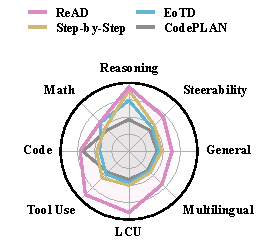
\includegraphics[width=0.45\columnwidth]{figure/rqX_radar_sota_vs_read_150m.pdf}
  \caption{ReAD beats SOTA baselines that are specifically designed for reasoning, code, and math capabilities consistently.}
  % \vspace{-1.2\baselineskip}
  \label{fig:radar}
\end{wrapfigure}

\textbf{ReAD beats SOTA baselines.}
To further validate ReAD against SOTA capability distillation baselines that are specifically designed for certain 
capabilities, we include three representative methods that are commonly used for specializing student models, one per capability: step-by-step distillation~\citep{hsieh2023stepbystep} for reasoning, Equation-of-Thought Distillation (EoTD)~\citep{zhu2024distilling} for math, and CodePLAN~\citep{sun2024enhancing} for code. For a fair comparison under our setting, we adapt each baseline to our LLaMa teacher-student pair and token budget as $150$M, and we distill the student using only the corresponding capability pool. We report the resulting capability profiles on all eight benchmarks using the same evaluation protocol as the main experiments in Figure~\ref{fig:radar}. The results show that these capability-targeted baselines mainly concentrate gains on their target capability and exhibit weaker transfer to other capabilities, producing an imbalanced profile that matches the interaction patterns observed in our empirical study. In contrast, ReAD achieves a consistently stronger and more balanced profile across capabilities, and it is never worse than these baselines on its target capability, while improving substantially on non-target capabilities.


% \subsection{Held-out Downstream Transfer}
% \label{sec:app_xstest}

\textbf{Held-out Downstream Transfer}. To test whether ReAD transfers beyond capability-aligned benchmark tasks, we
evaluate on XSTest using the same requirement identifier and allocation pipeline
without adding a new capability head. Lower safe-refusal and higher
unsafe-refusal scores are better.

\begin{table}[h]
  \centering
  \caption{
  Held-out XSTest evaluation. ``Best baseline'' denotes the best of the six
  SFT/KD baselines for each metric.
  }
  \label{tab:xstest}
  \scriptsize
  \setlength{\tabcolsep}{4pt}
  \renewcommand{\arraystretch}{0.95}

  \begin{tabular}{@{}lcccc@{}}
    \toprule
    \textbf{Method}
      & \textbf{20M safe $\downarrow$}
      & \textbf{20M unsafe $\uparrow$}
      & \textbf{150M safe $\downarrow$}
      & \textbf{150M unsafe $\uparrow$} \\
    \midrule
    Best baseline
      & $15.1\pm0.77$
      & $75.5\pm1.09$
      & $13.1\pm0.69$
      & $79.0\pm0.88$ \\
    \textbf{ReAD}
      & $\mathbf{13.8\pm0.72}$
      & $\mathbf{78.1\pm0.97}$
      & $\mathbf{11.8\pm0.58}$
      & $\mathbf{81.6\pm0.83}$ \\
    \bottomrule
  \end{tabular}
\end{table}

\section{Related Work}
\label{sec:relate}

\textbf{Capability Distillation for Large Language Models.}\label{sec:relate_kd}
Recent work on capability distillation has focused on transferring specific capabilities such as instruction following and context manipulation~\citep{taori2023stanford, chiang2023vicuna, peng2023instruction, xu2023wizardlm}, thinking patterns~\citep{zhang2024knowledgeable, cheng2023adapting}, or text and code generation capability~\citep{zhang2025recommendation, li2023starcoder}. These methods typically steer a teacher LLM via prompts or rationales, generate distillation data or logits, and fine-tune the student on that evidence. However, the majority of methods operate under the assumption that distilling one target capability or domain is sufficient and rarely analyze how that focused training influences broader capability interactions within the student model. To the best of our knowledge, ReAD is the first framework that explicitly accounts for capability interdependence during the distillation.

\section{Broader Impact}
\label{sec:broader_impact}

ReAD aims to make capability distillation more budget-efficient by allocating
limited training tokens across interdependent LLM capabilities. A positive
impact is that smaller student models can become more useful under fixed compute
budgets, potentially reducing deployment cost and improving access to LLM-based
systems in resource-constrained settings. ReAD also explicitly monitors
cross-capability transfer, which can help practitioners diagnose when improving
one capability degrades others.

At the same time, more efficient distillation may lower the cost of producing
specialized models with dual-use capabilities, such as code generation, tool use,
or instruction following. Distilled models may also inherit biases, unsafe
behaviors, privacy risks, or other limitations from teacher models and training
data. In addition, if the capability probes or task requirement vectors are
misaligned with the intended deployment objective, ReAD may optimize benchmark
utility while overlooking safety-, fairness-, or robustness-relevant behaviors.

We therefore view ReAD as a research framework rather than a deployment-ready
safety guarantee. For sensitive applications, practitioners should combine ReAD
with task-specific safety evaluation, robustness and bias audits, data filtering,
red-team testing, and monitoring of off-target capability changes. Any release
or deployment of distilled models should follow the usage restrictions of the
underlying models and include appropriate documentation of intended use,
limitations, and safety evaluations.

\section{Limitation and Future Work}

While ReAD improves budget efficiency by using low-cost capability monitoring and adaptive allocation, it still relies on two practical components that can limit performance. First, the task requirement estimator and the probe suite may be imperfect: if the inferred essential capabilities or probe signals are misaligned with true task utility, ReAD can allocate budget suboptimally. Second, our capability set and data generator are necessarily finite and template-driven, which may not cover all behaviors a real task depends on, especially for highly domain-specific or long-horizon tasks. Future work can address these limitations by learning more robust and transferable task requirement models, designing probe suites with stronger coverage and better calibration to task utility, and expanding capability definitions and data generation beyond templates (e.g., automatic discovery of capability axes and open-ended curriculum generation). Another promising direction is to jointly optimize allocation and student training dynamics (e.g., optimizer schedules and parameter-efficient adapters) under the same budget, and to extend ReAD to settings with distribution shift, multi-task deployment, or continual updates where requirements and transfer patterns evolve over time.